
%!TEX root =  NLPVision_proposal.tex

%\begin{figure}

\parbox{5.5in}{
\tiny
{\sf
The Bobolink (Dolichonyx oryzivorus) is a small New World blackbird and the only member of genus Dolichonyx.

\vspace{2pt}
Description: Adults are 16-18 cm (6-8 in) long with short finch-like bills. They weigh about 1 oz. Adult males are mostly black, although they do display creamy napes, and white scapulars, lower backs and rumps. Adult females are mostly light brown, although their coloring includes black streaks on the back and flanks, and dark stripes on the head; their wings and tails are darker. The collective name for a group of bobolinks is a chain.

\vspace{2pt}
Distribution and movement: These birds migrate to Argentina, Bolivia and Paraguay. One bird was tracked flying 12,000 mi over the course of the year, and up to 1,100 mi in one day. They often migrate in flocks, feeding on cultivated grains and rice, which leads to them being considered a pest by farmers in some areas. Although Bobolinks migrate long distances, they have rarely been sighted in Europe-like many vagrants from the Americas, the overwhelming majority of records are from the British Isles. 
Each fall, Bobolinks gather in large numbers in South American rice fields, where they are inclined to eat grain. This has earned them the name "ricebird" in these parts. However, they are called something entirely different in Jamaica (Butterbirds) where they are collected as food, being that they are very fat as they pass through on migration.


\vspace{2pt}
Behavior:
Their breeding habitats are open grassy fields, especially hay fields, across North America. In high-quality habitats, males are often polygynous. Females lay 5 to 6 eggs in a cup-shaped nest, which is always situated on the ground and is usually well-hidden in dense vegetation. Both parents feed the young. 
Bobolinks forage on or near the ground, and mainly eat seeds, insects, cultivated grains and rice.
Males sing bright, bubbly songs in flight; these songs gave this species its common name.
}}
\parbox{1.4in}{
\centering
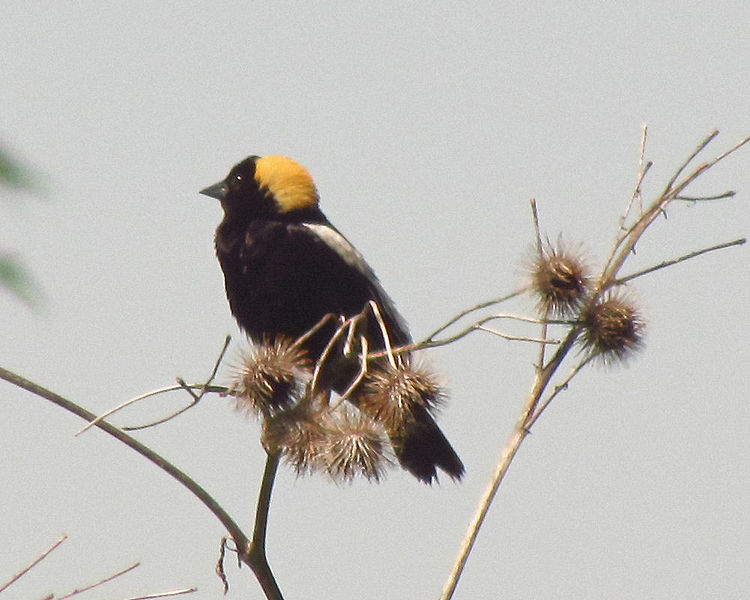
\includegraphics[width=1.2in]{Bobolink.jpg}
%\tiny {\sf (male)}
}
%\end{figure}
